%!TEX root = ../thesis.tex
%*******************************************************************************
%*********************************** First Chapter *****************************
%*******************************************************************************

\chapter{Introduction}  %Title of the First Chapter

\ifpdf
    \graphicspath{{Chapter1/Figs/Raster/}{Chapter1/Figs/PDF/}{Chapter1/Figs/}}
\else
    \graphicspath{{Chapter1/Figs/Vector/}{Chapter1/Figs/}}
\fi

\newcommand{\citetex}[1]{\citeauthor{#1} (\citeyear{#1})}
\newcommand{\citebrac}[1]{(\citeauthor{#1}, \citeyear{#1})}

%********************************** %First Section  ****************************
\section{Background}

Tremie methods for casting bored piles and diaphragm walls, {\bfseries figure \ref{fig:tremie_blank}}, require a specialist concrete termed 'tremie concrete'. In both fresh and cured state, this concrete must meet stringent Euro and British design codes. Despite these regulations however, problems within the final product are still prevalent throughout the industry. In 2014 the European Federation of Foundation Contractors and the Deep Foundation Institute set up a task-group wherein the primary aim was to develop a clearer understanding of the root cause of these issues. The task group hypothesised that inadequate workability and stability of the concrete was in part caused by the inability of current design guidelines to predict when problems are likely to occur, \citetex{EFFC}.\\

\noindent
In order to provide evidence to support this hypothesis, two avenues of investigation have arisen. Namely, a practical approach as seen by \citetex{bjorn}  and a simulative approach as described in this paper.\\

\noindent
Along side an analysis of the issues to be investigated, a comprehensive review of literature surrounding fresh concrete and its ability to be modelled accurately is presented, followed by a potential methodology of investigation. 

\begin{figure}[H]
\centering
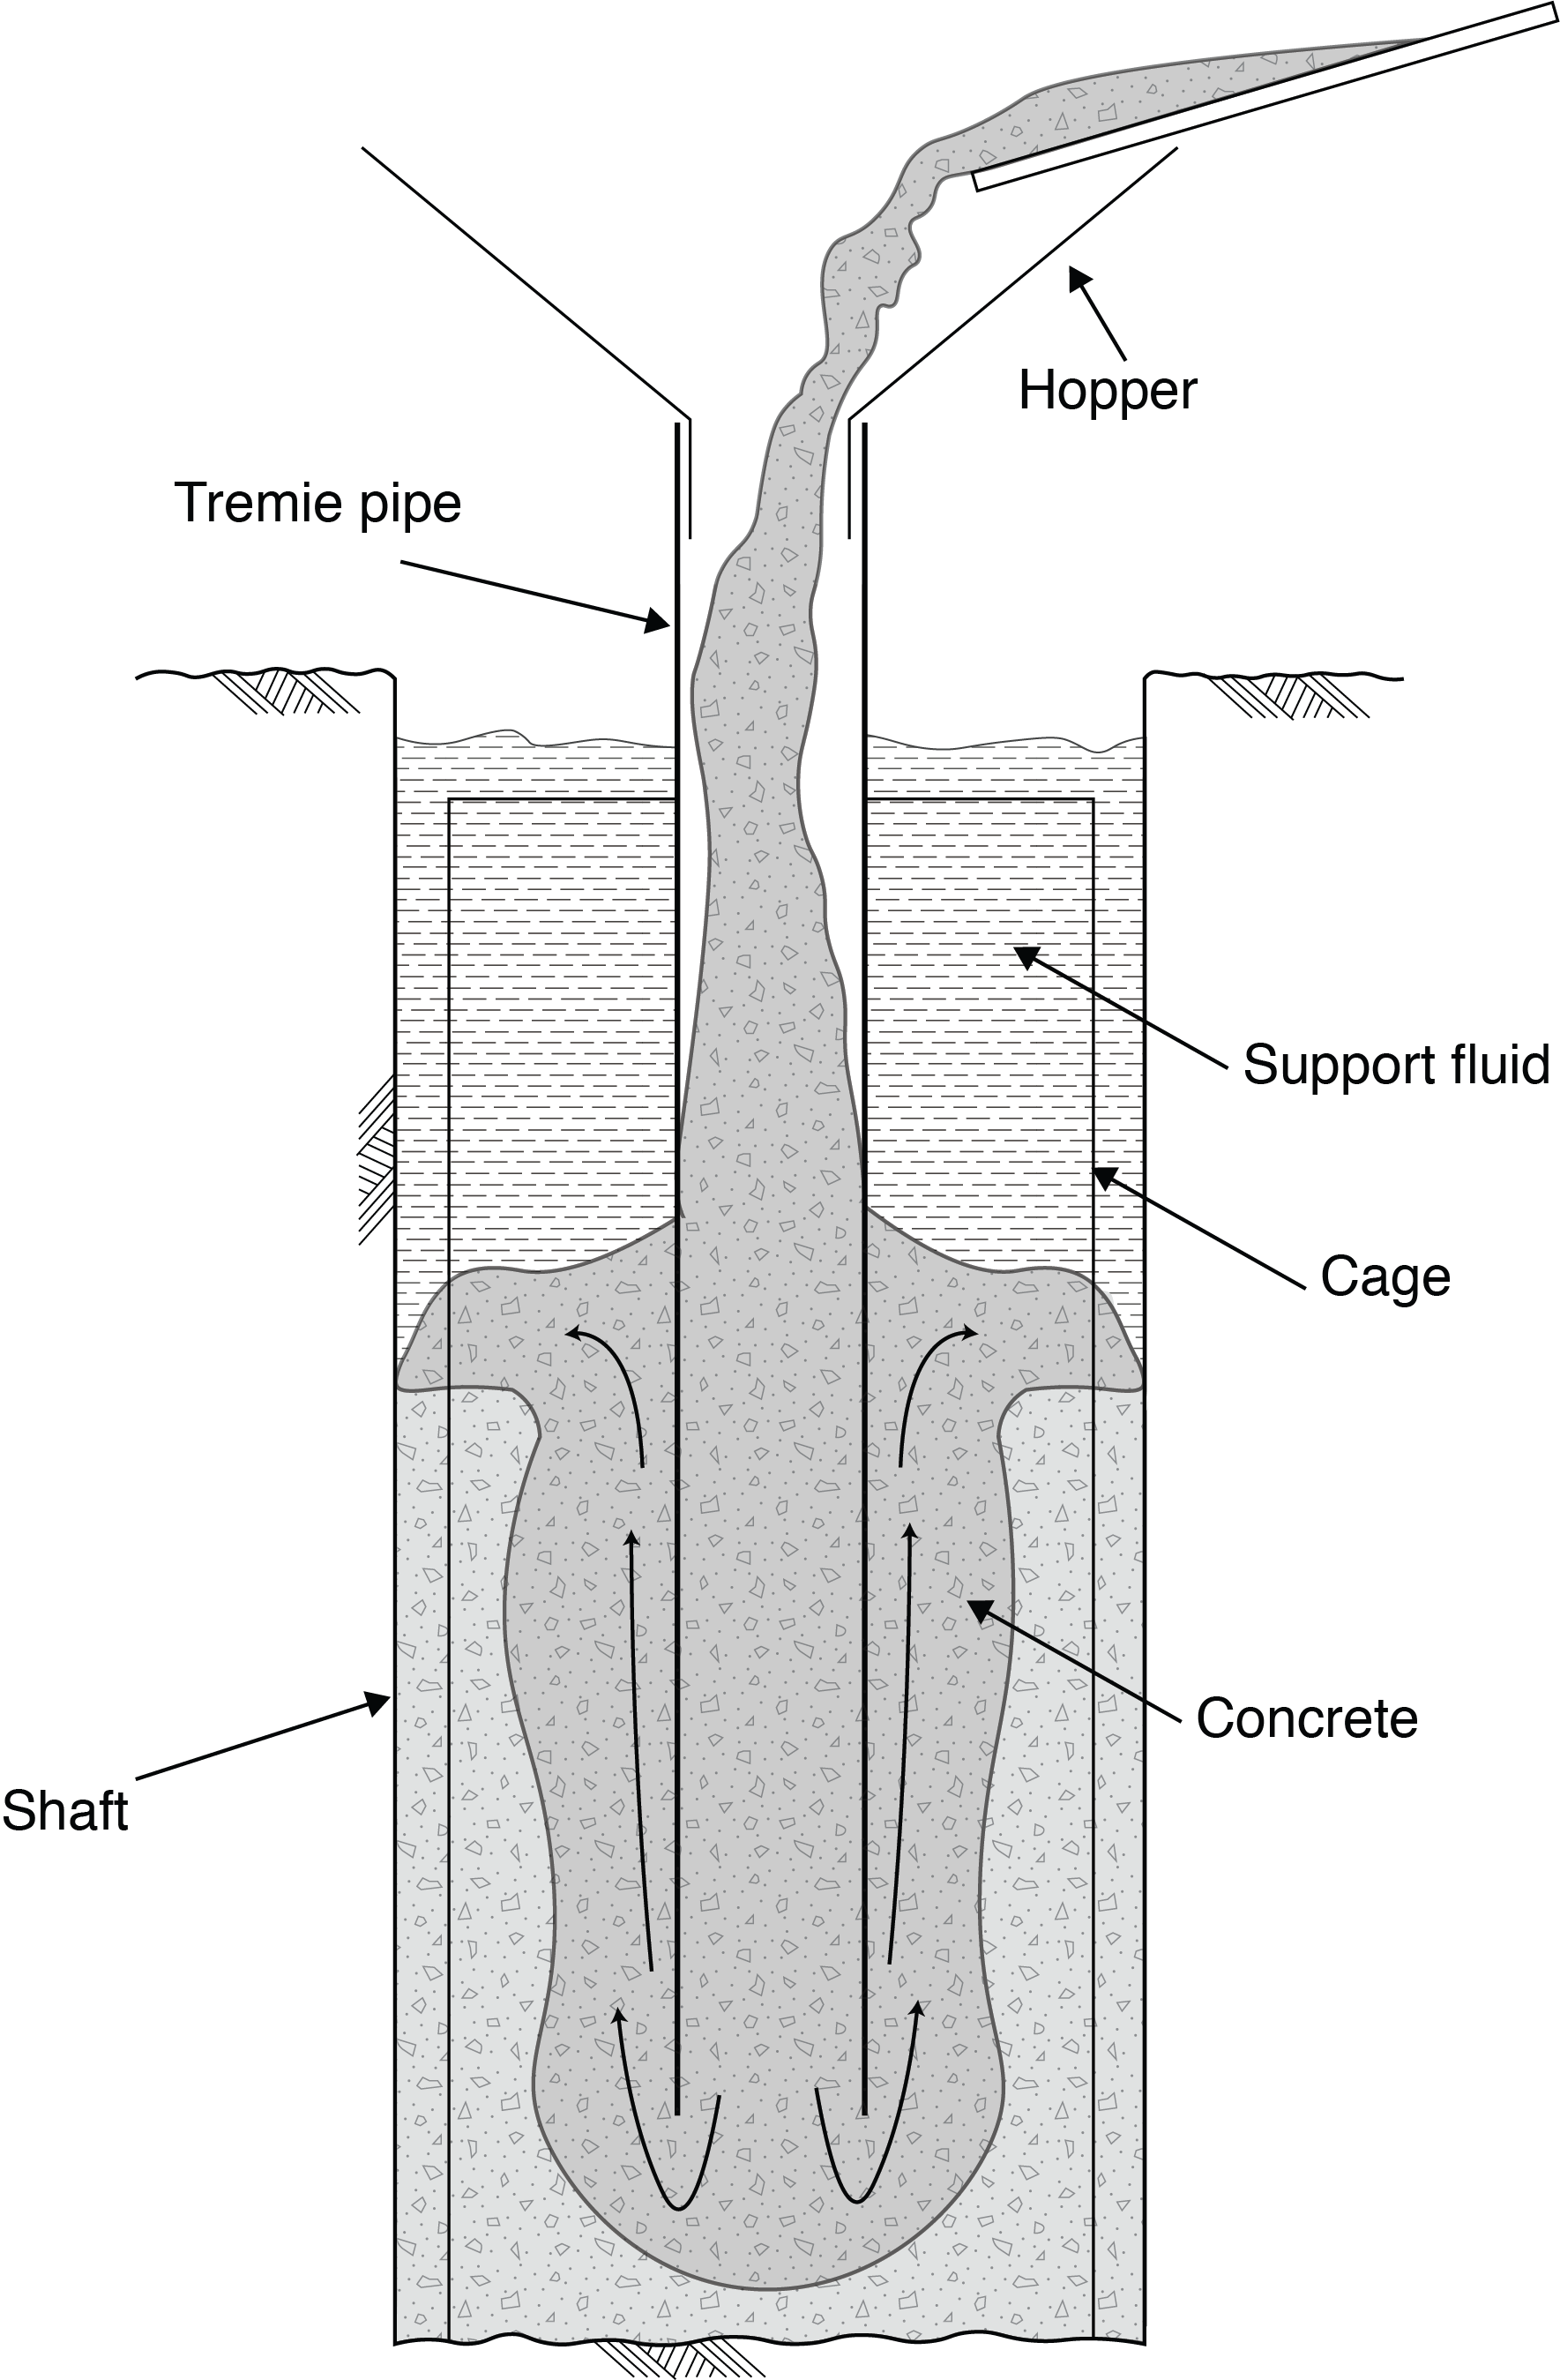
\includegraphics[width=0.7\textwidth]{tremie_blank.png}
\caption{\label{fig:tremie_blank} Schematic diagram of a tremie method for emplacing concrete under a support fluid within a bored pile(not to scale).}
\end{figure}

\section{Research Objectives}
Coalescing all issues relating to tremie concrete into the same simulation is unlikely to produce any significant findings. A more pragmatic approach would be to assess each identified variable in the process individually, making a judgement it's impact on the final result.\\

\noindent
In this study, the impact of tremie method equipment shown in {\bfseries figure \ref{fig:tremie_blank}} is considered along side the resultant behaviour of the concrete, especially its dominant flow pattern. The change in behaviour of the concrete with changing variables will be documented in order to advise how best to avoid any issues that arise. Although there are some areas of investigation involving the tremie pipe, the dimensions and centring of the pipe as specified by EN 1536:2010 are not considered. 


\section{Areas of Investigation}

When analysing the tremie method, each area of investigation falls within one of three subdivisions; initiation of concrete flow, during concrete flow, and bleed and segregation, {\bfseries figure \ref{fig:tremie_colour}}.

\begin{figure}[H]
\centering
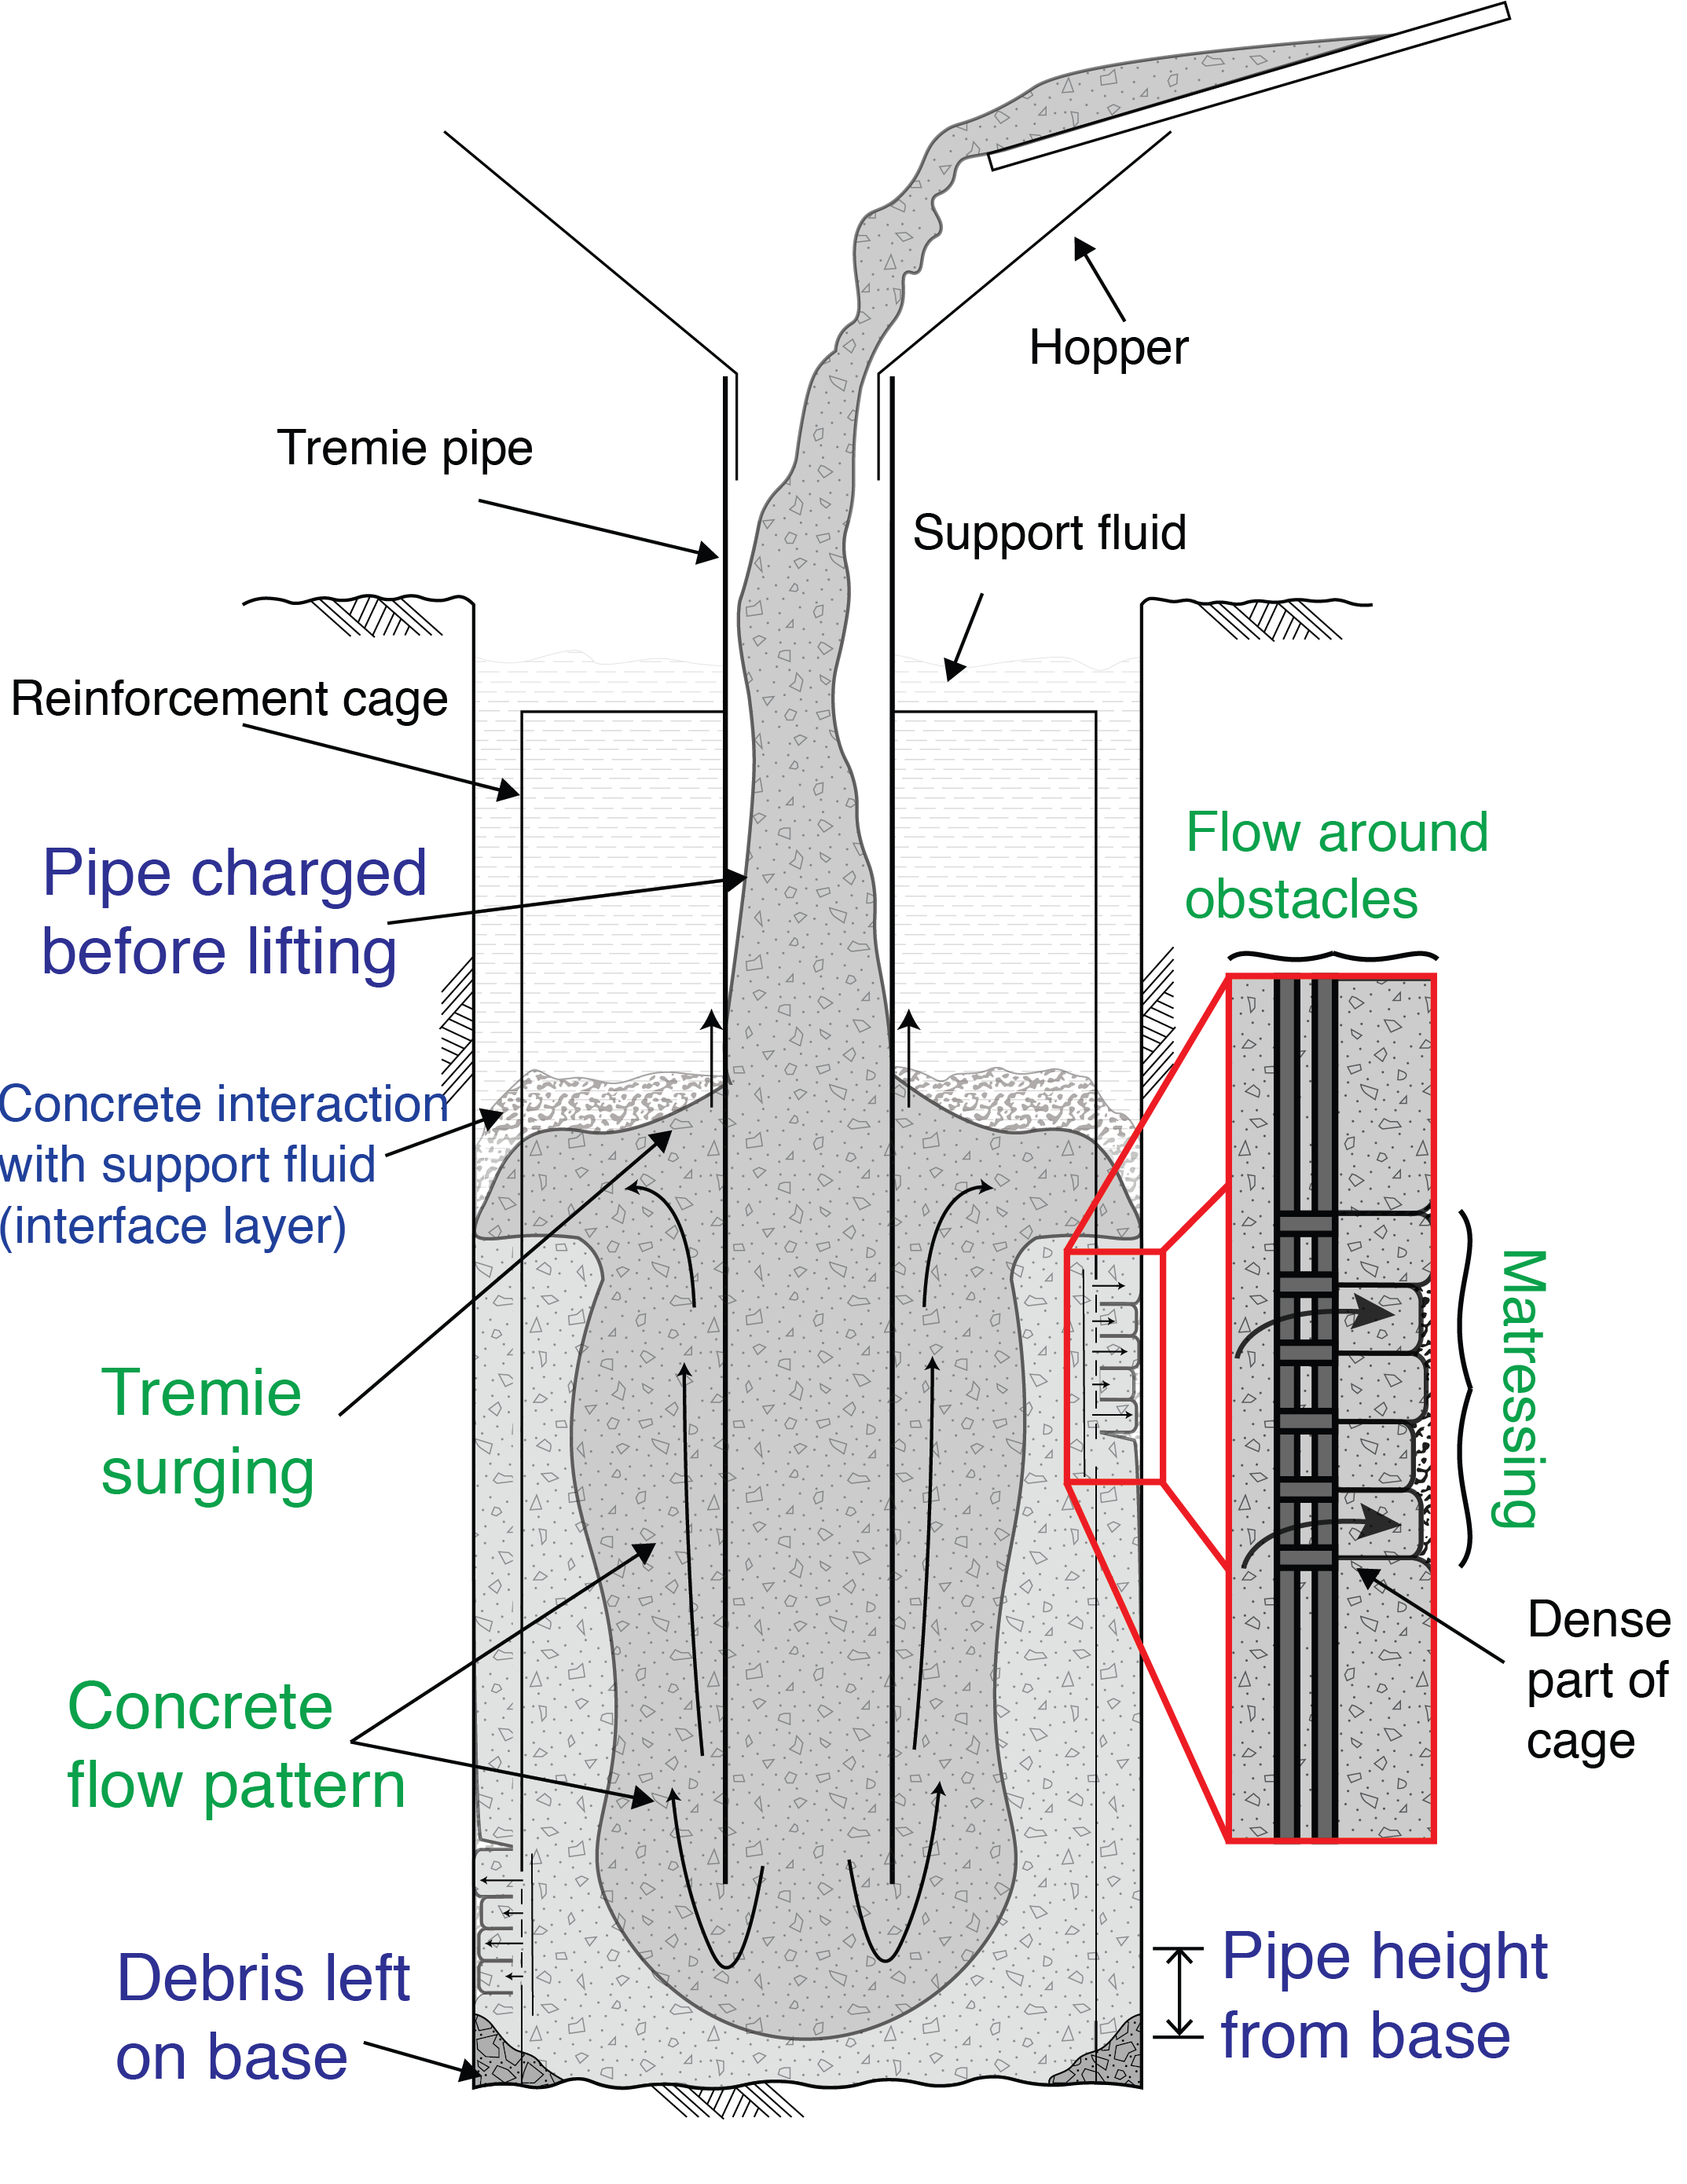
\includegraphics[width=0.65\textwidth]{tremie_colour.png}
\caption{\label{fig:tremie_colour} Schematic diagram of a bored pile cast using tremie method, with areas of investigation highlighted and colour coded.}
\end{figure}


\subsection{Initiation of Concrete Flow}

Areas of investigation related to the initiation of concrete flow are centred around the physical apparatus used in the process and the conditions of the shaft prior to beginning concreting as seen in {\bfseries figure XX}.\\

\noindent
The importance of base cleaning, demonstrated in {\bfseries figure XX}, is reiterated throughout \citeauthor{BS1536}, \citetex{EFFC}, and \citetex{Sperwall}. The regular need for pile baring capacity to be accurately calculated by relying on the assumption of a smooth base being a primary concern. However, although a smooth base is critical for pile design purposes, \citetex{EFFC} hypothesise that debris from the base can be stirred up and included in the pile. Developing a simulation to assess the degree of inclusions caused by an unclean base could provide advice on whether base cleaning is needed in conditions where end baring capacity is not a critical factor of the pile design.\\

\noindent
{\bfseries Figure XX b} and {\bfseries Figure XX c} demonstrate the initial charging and raising of the tremie to initiate concrete flow. \citetex{Sperwall} recommend raising the pipe to $200mm$ prior to initiation of flow to allow for the prevention of blockages from the initial pour. Both \citetex{Sperwall} and \citetex{EFFC} also recommend the use of a plug to allow the tremie to be filled with concrete prior to initiation and to prevent contamination of the concrete with support fluid during filling of the pipe. However, little evidence is provided to determine the effectiveness of using such a method. This study aims to simulate varying plugging methods and make a recommendation on the effectiveness of each. 




















